\section{Caches}

\begin{figure}
    \centering
    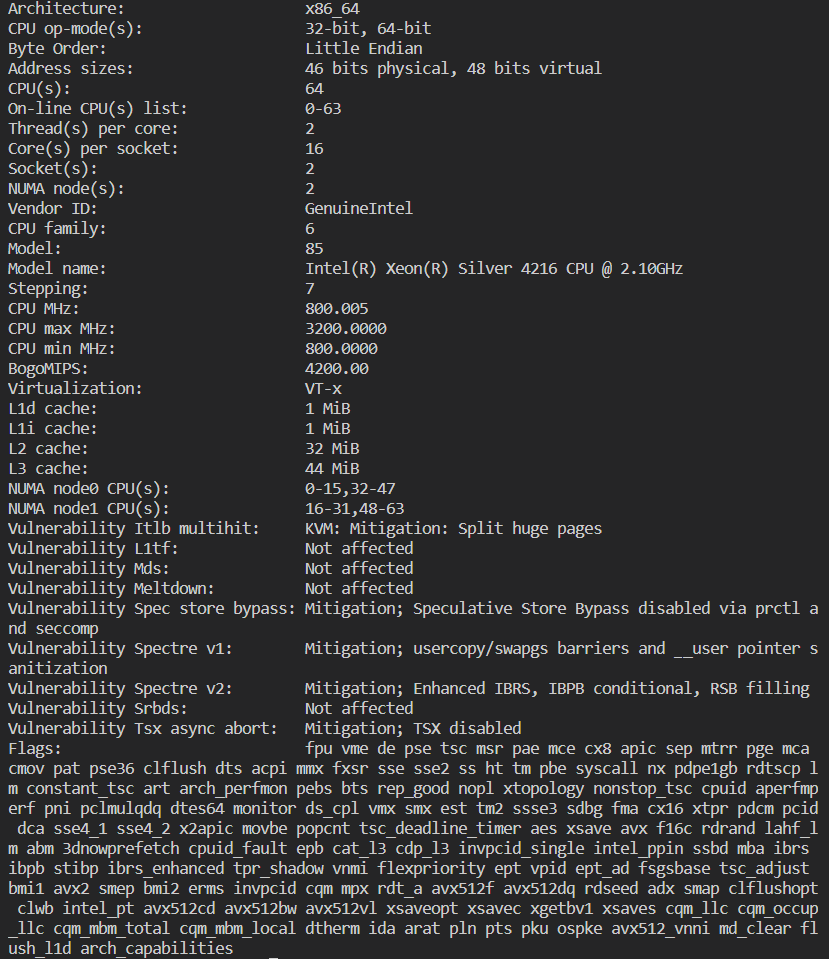
\includegraphics[scale=0.8]{imgs/lscpu.png}
    \caption{\label{fig:lscpu}
        계산 노드에서의 \texttt{lscpu} 명령어의 출력 결과.
    }
\end{figure}

Fig.~{\ref{fig:lscpu}}과 같이 계산 노드의 CPU 정보를 얻었다.

\begin{enumerate}[label= (\alph*)]

    \item {
        CPU의 모델명은 Intel(R) Xeon(R) Silver 4216 CPU @ 2.10GHz 이고,
        microarchitecture는 Cascade Lake이다.
    }

    \item {
        L1 data cache는 32KB이다. 각 코어에 하나씩 존재한다.
        총 16개의 코어가 존재하므로 L1 data cache의 총 용량은 32KB $\times$ 16 = 512KB 이다.
        L2 cache는 1MB이다. 각 코어에 하나씩 존재한다.
        총 16개의 코어가 존재하므로 L2 cache의 총 용량은 1MB $\times$ 16 = 16MB이다.
        L3 cache는 22MB이다. L3 cache는 모든 코어가 공유한다\cite{CPUWorld,SpecOrg}.
    }

    \item {
        L1 data cache, L2 cache, L3 cache 모두 write-back cache이다\cite{WikiChip}.
    }

    \item {
        L1 data cache는 8-way set associative, L2 cache는 16-way set associative,
        L3 cache는 11-way set associative cache이다.
        또한 한 cache line은 모든 cache에서 64B이다\cite{CPUWorld,WikiChip}.
        
        L1 data cache의 하나의 set의 크기는 $32 \div 8 = 4$KB이다.
        따라서 한 set에는 64개의 cache line이 존재한다.
        L2 data cache의 하나의 set의 크기는 $1024 \div 16 = 64$KB이다.
        따라서 한 set에는 1,024개의 cache line이 존재한다.
        L3 data cache의 하나의 set의 크기는 $22 \times 1024 \div 11 = 2048$KB이다.
        따라서 한 set에는 65,536개의 cache line이 존재한다.
    }
    
\end{enumerate}